\chapter{Machine Learning}
\label{ch:neural-network}

In this Chapter we will see how machine learning techniques can be successfully applied to solve financial problems. We first do a quick tour on the theory behind neural networks and then see few examples and practical applications regarding regression and classification issues.

Beware that this Chapter just scratches the surface of machine learning theory which has seen a huge development in the latest years leading to thousands of applications in many different fields.
    
\section{Neural Networks}\label{neural-networks}

Artificial Neural Networks (ANN or simply NN) are information processing models that are developed by inspiring from the working principles of the human brain. Their most essential property is \emph{the ability of learning from sample sets}.

\subsection{Neurons and Activation Functions}
The basic unit of an ANN is the neuron.
It consists of weights (\(w_i\)) and takes in input real numbers (\(x_i\)). After the injection into a neuron all these inputs are individually weighted, added together (sometimes it is added also a bias \(w_0\)) and passed into the activation function which produces the final neuron output

\[ \textrm{Inputs} = \sum_{i=1}^{N} x_i w_i + w_0 \rightarrow f(\textrm{Inputs}) = \textrm{Outputs}\]
Figure~\ref{fig:neuron} shows an example.

There are many different types of activation functions, examples are
\begin{itemize}
\item \emph{step function}: which returns just 0 or 1 according to the input value;
\item \emph{sigmoid}: which can be thought of as the continuous version of the step function, see Fig.~\ref{fig:act_func};
\item \emph{Rectified Linear Unit} (ReLU);
\item \emph{hyperbolic tangent} (tanh).
\end{itemize}

For a deeper discussion on activation functions see~\cite{bib:activation_function}.

\begin{figure}[htb]
\centering
\subfloat[Model of an artificial neuron.\label{fig:neuron}]{%
	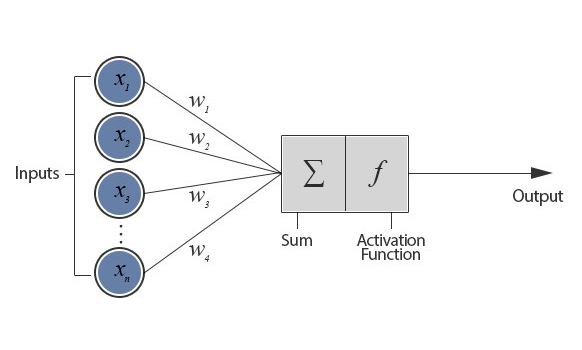
\includegraphics[width=0.6\textwidth]{figures/neuron}
}
\subfloat[Examples of sigmoidal and step activation functions.\label{fig:act_func}]{%
	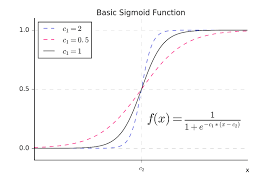
\includegraphics[height=0.30\textwidth]{figures/sigmoid}
}
\caption{Basic components of a neuron.}
\label{fig:sigmoid}
\end{figure}

\subsection{Training of a Neuron}
\label{training-of-a-neuron}

When teaching children how to recognize a bus, we just tell them, showing an example: "This is a bus. That is not a bus." until they learn the concept of what a bus is. Afterwards, if a child sees new objects that she hasn't seen before, we could expect her to recognize correctly whether the new object is a bus or not.

This is exactly the idea behind neuron training. Inputs from a \emph{training} set are presented to the neuron,  one after the other, together with the correct output. During the process neuron weights are modified so that its response best matches the true output.

When an entire pass through all of the inputs is completed (an \emph{epoch}) the neuron has learned. Usually to make it learn even better the same training data is processed multiple times.

After the training is completed, when an input vector \(\mathbf{x}\), contained in the training set, is presented to the neuron, it will output the correct value. If \(\mathbf{x}\) is not in the training set, the neuron will respond with an output close to those corresponding to other training vectors similar to \(\mathbf{x}\).

This kind of training is called \emph{supervised} because the input dataset is accompanied by the known targets (the true outputs), and we want our model to learn to predict the target from those input variables.

Unfortunately using just a neuron is not too useful since with such a simple architecture is not possible to solve the interesting problems we would like to face. 
The next step is to put together more neurons in \emph{layers}.

\subsection{Multilayered Neural Networks}
\label{multi-layered-neural-networks}

In a multilayered configuration each neuron from the \emph{input layer} is fed up to each node in the next \emph{hidden layer}. This kind of connection is repeated for each node down to the \emph{output layer}. 
We should note that there can be any number of nodes per layer and there are usually multiple hidden layers to pass through before ultimately reaching the output layer. The only two architectural constraints are on the neuron number in the input layer, that has to match the number of inputs, and on the nodes in the output layer which depends on the kind of target. Figure~\ref{fig:multilayered_nn} shows an example of such an architecture.

\begin{figure}[htb]
\centering
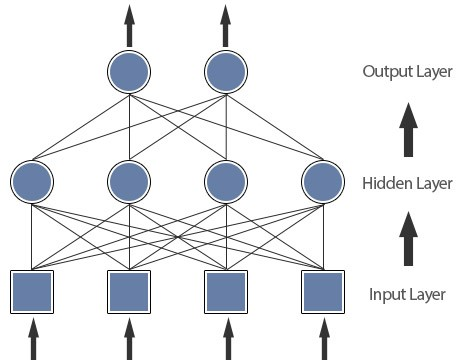
\includegraphics[width=0.6\textwidth]{figures/multilayer.jpeg}
\caption{A multilayered neural network.}
\label{fig:multilayered_nn}
\end{figure}

\subsection{Training a Multilayered Neural Network}
\label{training-a-multilayered-neural-network}

The training of a multilayered NN follows these steps:

\begin{itemize}
\tightlist
\item present an input sample to the neural network whose neurons are initialized with random weights;
\item compute the network output obtained by calculating the activation functions of each layer;
\item calculate the \emph{error (loss)} as the difference between NN predicted and target output;
\item re-adjust the network weights such that the error decreases;
\item continue the process for the entire sample (and also for several epochs), until the error is not changing too much (i.e. the process converged).
\end{itemize}
In Figure~\ref{fig:training} an example of training is shown.

\begin{figure}[htb]
\centering
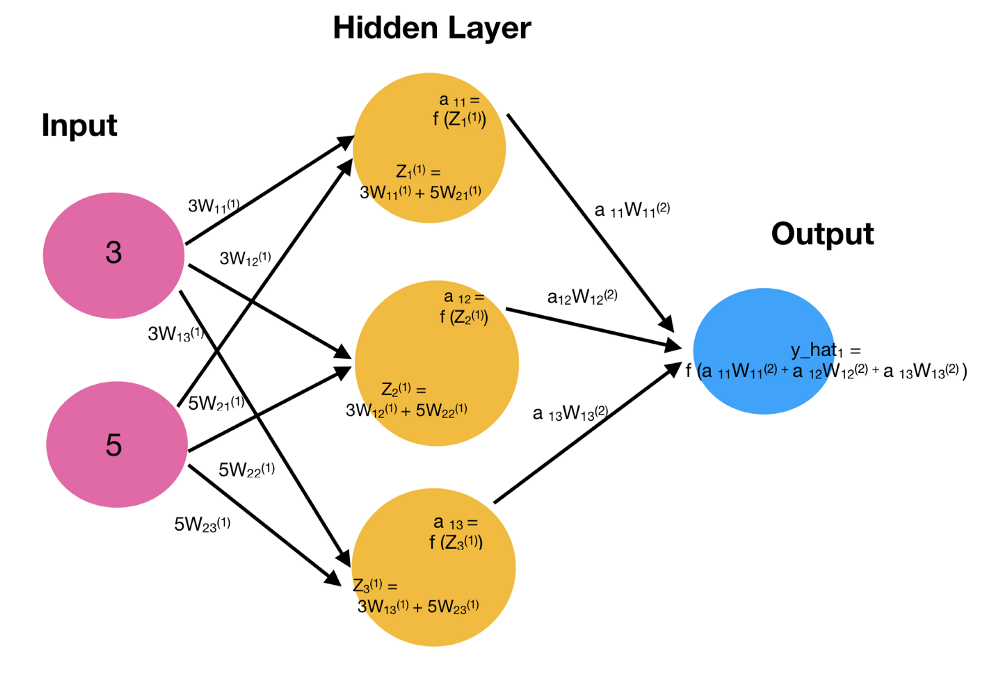
\includegraphics[width=0.9\textwidth]{figures/training_nn}
\caption{Training example of a multilayered neural network.}
\label{fig:training}
\end{figure}

\subsubsection{Loss Function}
The NN error is computed by the \emph{loss function}. Different loss functions will give different error estimates for the same prediction, and thus they have a considerable effect on the performance of any model. Two are the main choices

\begin{itemize}
\tightlist
\item Mean Absolute Error (MAE): the average of the absolute value of the differences between the predictions and true values. It shows how far off we are on average from the correct value. 
\item Root Mean Squared Error (MSE): the square root of the average of the squared differences between the predictions and true values. It instead penalizes larger errors more heavily and is commonly used in regression tasks. 
\end{itemize}

Either metrics may be appropriate depending on the situation and you can use both for comparison. 
More information about loss function can be found in~\cite{bib:loss_function}.

\subsubsection{Back-propagation}
The loss is a function of the internal parameters of the model (i.e neuron weights). For an accurate predictions, one needs to minimize the calculated error and in a neural network, this is done using
\emph{back-propagation}~\cite{bib:backpropagation}.

In this algorithm the current error is "propagated" backwards to previous layers, where it is used to modify the weights in such a way that the loss tends to be minimized.
The weights are modified with a function called \emph{optimization function} (we will use \emph{Adam} in the following but there are more).

\subsection{Regression and Classification}
\label{regression-and-classification}

The two main categories of problems that can be solved with neural networks are \emph{classification} and \emph{regression}. Let's see their characteristics and differences.

\subsubsection{Classification}
\label{classification}

Classification is the process of finding a function which helps in dividing the input dataset into classes based on its characteristics. 
The goal is to find the mapping function between the input (\(x\)) and the \textbf{discrete} output (\(y\)) or in other words to find the decision boundary, which can divide the dataset into the different classes.

A typical classification problem is the \emph{email spam detection}. The model is trained on different parameters using millions of emails, and whenever it receives a new email, it checks whether is spam or not. Classification algorithms can also be used in speech recognition, car plates identification, \ldots

\subsubsection{Regression}
\label{regression}

Regression is the process of finding hidden correlations between dependent variables. It helps in predicting market trends, house prices, \ldots

The goal is to find the mapping function between the input variables (\(x\)) and the \textbf{continuous} output variable (\(y\)), that is to find the best fit which can predict the output.

As an example suppose we want to do weather forecasting. The model is trained on past data, and on the basis of today's inputs can predict the weather for future days. In general whenever we are dealing with function approximations this kind of algorithms can be applied.

\begin{attention}
\subsubsection{Technical Note}
\label{technical-note}

Neural network training and testing is performed using two modules: \texttt{keras}~\cite{bib:keras} (which in turn is based on a Google open source library called \texttt{tensorflow}~\cite{bib:tensorflow}) and \texttt{scikit-learn}~\cite{bib:scikit} which provide many useful utilities.

In order to hide as much as possible the many little subtleties of a NN implementation it has been developed a class (\texttt{FinNN}) which is a wrapper for \texttt{keras} functionalities and should make the whole process easier.
\end{attention}

\section{Function approximation}
\label{function-approximation}

Let's design an ANN which is capable of learning the functional form underlying a set of data. The implementation of the neural network starts by importing the necessary modules.

\begin{ipython}
from finnn import FinNN
import numpy as np
\end{ipython}

The training sample is generated as a two columns array: \(x\) (input), \(f(x)\) (target output) where \(f(x) = x^3 +2\). 

Before embarking into the training the sample undergoes to a simple transformation in order to have all the inputs and outputs in the \([0, 1]\) range. This transformation is called \emph{normalization}, and is done to provide the NN with "equalized" inputs since it could be fooled by very large or small numbers giving unstable results.

\begin{ipython}
x = np.array([i for i in np.arange(-2, 2, 0.001)])
y = np.array([i**3+2 for i in x])
print("Distribution of original data ", x.min(), x.max(), y.min(), y.max())

trainer = FinNN("ANN")
# define input and output and fraction of testing sample
trainer.setData(x, y, test_size=0.2)
trainer.normalize()
print("The same data after the normalization ", trainer.x.min(),
       trainer.x.max(), trainer.y.min(), trainer.y.max())
\end{ipython}
\begin{ioutput}
Distribution of original data  -2.0 1.9989999999995596 -6.0 9.98800599899472
The same data after the normalization  0.0 1.0 0.0 0.9999999999999999
\end{ioutput}

\subsection{Neural Network Design}
\label{neural-network-design}

There is no rule to guide developers into the design of a neural network in terms of number of layers and neurons (the so called \emph{hyper-parameters}). 

One popular method for hyper-parameter optimization is the \emph{grid search}. 
A list of possible values for each hyper-parameter is defined, then the model is run multiple times, each time with a different combination of the hyper-parameter values. In the end the set giving the best result is taken. This is the most thorough way of selecting the neural network architecture but it is also the most computationally intense.
In the end a \emph{trial and error} strategy is what is implemented anyway, and the solution giving the best accuracy is selected although without an exhaustive check of all the possibilities.

In general a larger number of nodes is better to catch highly structured data with a lot of feature although it may require larger training sample to work correctly.

As a rule of thumb a NN with just one hidden layer with a number of neurons averaging the inputs and outputs is sufficient in most cases.

In the following we will use complex networks just for illustration, but no attempt in optimizing the layout has been done at all.

Here two layers with 15 and 5 neurons respectively and a \texttt{tanh} activation function are used, see Fig,~\ref{fig:ann_1}. The \texttt{inputs} parameter has to be set to 1 since we have just one single input, the \texttt{x} value.

\begin{ipython}
# design the neural network model
trainer.addInputLayer(inputs=1, neurons=15, activation='tanh')
trainer.addHiddenLayer(neurons=5, activation='tanh')
trainer.addOutputLayer(outputs=1)

# define the loss function (mean squared error)
# and optimization algorithm (Adam)
trainer.compileModel(loss='mse', opt='adam')

# fit the model on the training dataset
trainer.fit(epochs=2000, verbose=1)
\end{ipython}
\begin{ioutput}
Epoch 1/2000
3200/3200 [==============================] - 0s 31us/step - loss: 0.2362
Epoch 2/2000
3200/3200 [==============================] - 0s 6us/step - loss: 0.1498
...
Epoch 1999/2000
3200/3200 [==============================] - 0s 18us/step - loss: 8.7152e-06
Epoch 2000/2000
3200/3200 [==============================] - 0s 17us/step - loss: 5.9604e-06
\end{ioutput}

\begin{figure}[htb]
\centering
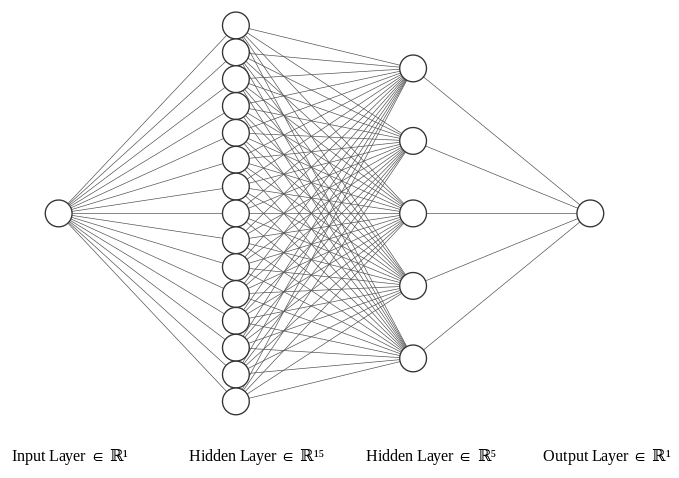
\includegraphics[width=0.9\textwidth]{figures/ann_1.png}
\caption{Graphical representation of the ANN used to approximate the function $f(x) = x^3 + 2$.}
\label{fig:ann_1}
\end{figure}

The output shows a counter with the current epoch number and the computed loss which is evaluated using the method chosen in the code.

When the training is completed we can evaluate how good it is. \textbf{Usually performance is measured using the loss function value at the end of the training.}
This can be done with the \texttt{evaluate()} method

\begin{ipython}
trainer.evaluate()
\end{ipython}
\begin{ioutput}
3200/3200 [==============================] - 0s 83us/step
Training: 6.1983578859781115e-06
800/800 [==============================] - 0s 52us/step
Test: 6.47684617433697e-06
\end{ioutput}
\noindent

A \emph{perfect} prediction would have led to \(\textrm{loss}=0\) so the lower this number the better is our training. 

Model performance improves with the number of epochs in the training, since the NN has more chances to learn the input features. To get an idea of what is going on in Fig.~\ref{fig:training_vs_epochs} are shown the actual function we want to approximate and different predictions obtained with the same NN architecture but various number of epochs (i.e. 5, 100, 800, 5000) in the training.

\begin{figure}[htb]
\centering
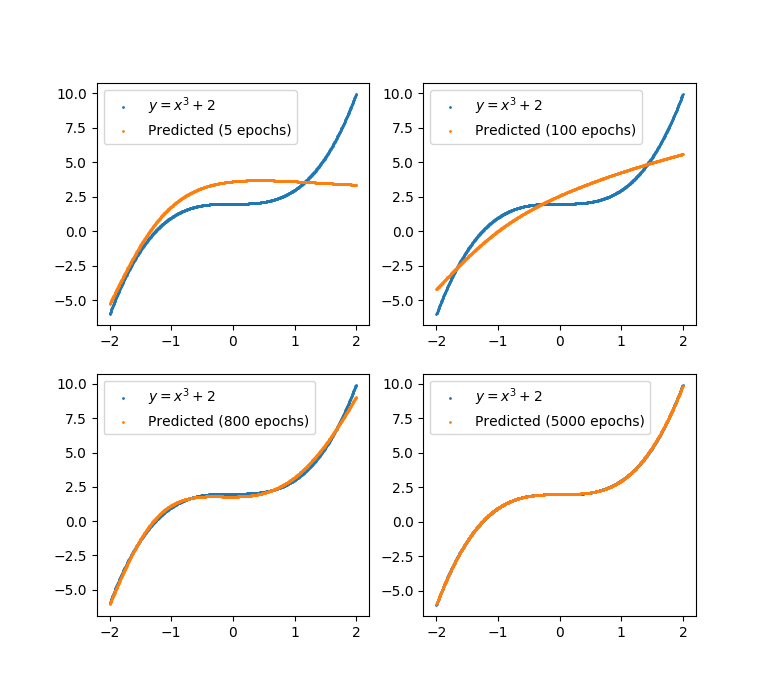
\includegraphics[width=0.9\textwidth]{figures/training_vs_epoch}
\caption{Prediction of the target $f(x)$ using different number of epochs in the training (5, 100, 800 and 5000) respectively.}
\label{fig:training_vs_epochs}
\end{figure}

\subsection{Overtraining}
A common issue to avoid during the training is \emph{overtraining} or \emph{overfitting} a NN. 

This happens when a model is "trained too well" on the dataset. This means that the model mostly memorized data, and its performance accounts for a large accuracy within it but a low accuracy in similar but independent datasets. 

To check for overfitting it is required to split the available sample in at least two parts: training and testing (e.g.~80\% and 20\%) and to use the former to perform the training and the latter to cross-check the performance.

%Actually you should split the sample in three parts: training, testing and validation. What you would usually do is take the model with the highest validation accuracy and then test the model with the testing set.
%This makes sure that you don’t overfit the model. Using the validation set to choose the best model is a form of data leakage (or “cheating”) to get to pick the result that produced the best test score out of hundreds of them. Data leakage happens when information outside the training data set is used in the model.
%In this case, our testing and validation set are the same, since we have a smaller sample size.

Looking at the output of the \texttt{evaluate()} call we can compare the loss computed with the training sample to that on the testing sample. If the two numbers are comparable the NN is ok, otherwise if the loss on the training is much smaller than the testing we had overfitting.
In our example since the two numbers are in good agreement we can be confident that there hasn't been overtraining.

In case one would need more accuracy and had already incremented too much the number of epochs could either increase the training sample size or change the NN architecture.

\subsection{Black-Scholes call options}
\label{black-scholes-call-options}

The first financial machine learning application concerns European call options pricing: we will implement a neural network capable of approximate the Black-Scholes pricing formula

\begin{equation} 
P_\textrm{call} = F_\textrm{BS}(M, r, \sigma, \mathrm{ttm})
\end{equation}

The first step consists of generating the training sample, made of volatility ($\sigma$)-rate ($r$) pairs (for simplicity we set moneyness ($M$) and time to maturity (ttm) to 1). The target value is the call price, computed using the BS function.

\begin{ipython}
import pandas as pd
from finmarkets import call_m

data = []
for r in np.arange(0.01, 0.11, 0.001):
    for sigma in np.arange(0.1, 0.6, 0.005):
        call_price = call_m(1, r, sigma, 1)
        data.append({rate:r, "vol":sigma, "price":call_price])

df = pd.DataFrame(data)
df.to_csv("bs_training_sample.csv")
print (df.describe())
\end{ipython}
\begin{ioutput}
	rate           vol         price
	count  10000.000000  10000.000000  10000.000000
	mean       0.059500      0.347500      0.165274
	std        0.028868      0.144338      0.055387
	min        0.010000      0.100000      0.044852
	25%        0.034750      0.223750      0.119389
	50%        0.059500      0.347500      0.165476
	75%        0.084250      0.471250      0.212097
	max        0.109000      0.595000      0.277071
\end{ioutput}

Since it takes some time to generate data samples, it is always advisable to save them in a file since it may be needed to load it many times during the NN development. 

\textbf{Beware that this time we have TWO input parameters (rate and volatility)}. See Figure~\ref{fig:ann_2} for a graphical representation of the designed ANN.

\begin{figure}[htb]
\centering
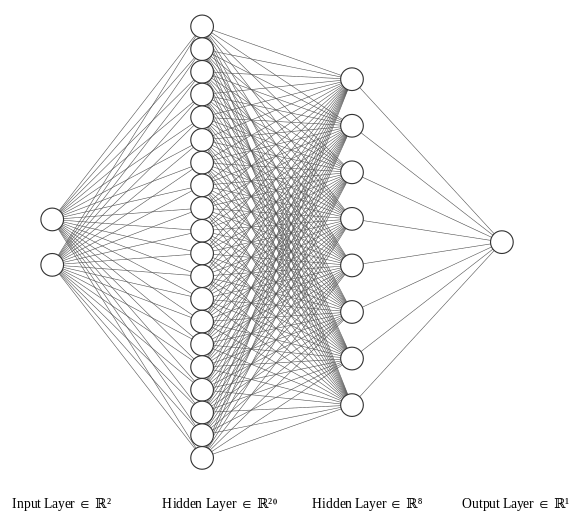
\includegraphics[width=0.9\textwidth]{figures/ann_2.png}
\caption{Graphical representation of the ANN used to approximate the Black and Scholes oprion price function.}
\label{fig:ann_2}
\end{figure}

\begin{ipython}
data = pd.read_csv("bs_training_sample.csv")
x = data.loc[:, ['rate', 'vol']].values
y = data.loc[:, 'price'].values

trainer = FinNN("ANN")
trainer.setData(x, y, test_size=0.20)
trainer.normalize()
trainer.addInputLayer(inputs=2, neurons=20, activation='relu')
trainer.addHiddenLayer(neurons=8, activation='relu')
trainer.addOutputLayer(outputs=1)

trainer.compileModel(loss='mse', opt='adam')
trainer.fit(epochs=3000, batch_size=500, verbose=1)
\end{ipython}
\begin{ioutput}
Epoch 1/3000
8000/8000 [==============================] - 0s 16us/step - loss: 0.3216
Epoch 2/3000
8000/8000 [==============================] - 0s 4us/step - loss: 0.2620
...
Epoch 2999/3000
8000/8000 [==============================] - 0s 4us/step - loss: 3.7983e-07
Epoch 3000/3000
8000/8000 [==============================] - 0s 3us/step - loss: 3.6476e-07
\end{ioutput}
\begin{ipython}
trainer.evaluate()

# when the training takes some time it is useful
# to save the model weights in a file to use it later on
trainer.saveModel('black_scholes')
\end{ipython}
\begin{ioutput}
8000/8000 [==============================] - 0s 52us/step
Training: 5.567638540924235e-07
2000/2000 [==============================] - 0s 44us/step
Test: 5.582978365055169e-07
\end{ioutput}

As you can see the training and testing samples give roughly the same loss value so we can be reasonably sure that there hasn't been \emph{overfitting}.
After the training is completed we can evaluate graphically how good it is by plotting the difference between predicted and actual output as a function of the input parameters, see Fig.~\ref{fig:vol_rate}. 

\begin{figure}[htb]
\centering
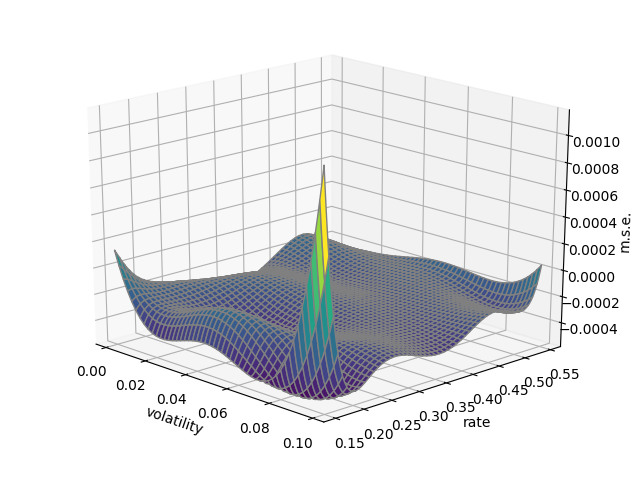
\includegraphics[width=0.7\textwidth]{figures/vol_rate}
\caption{Mean squared error as a function of volatility and rate for our Black-Scholes function prediction.}
\label{fig:vol_rate}
\end{figure}

Say we want to know the price of an at the money, 1 year call when the risk-free rate is 0.015 and the underlying volatility 0.234:

\begin{ipython}
import numpy as np
from finmarkets import call_m

# here we load the trained model
trainer.loadModel('black_scholes')

# this is our input vector
rv = np.array([[0.015, 0.234]])
# here we compare the predection with the BS call price

print ('{} => {:.4f} (expected {:.4f})'.format(rv.tolist(),
                                               trainer.predict(rv)[0][0],
                                               call_m(1, rv[0][0], rv[0][1], 1)))
\end{ipython}
\begin{ioutput}
[[0.015, 0.234]] => 0.1001 (expected 0.1001)
\end{ioutput}

It is very important to remember that a \textbf{NN cannot extrapolate}.
Indeed if you try to predict the price of a call from rate and volatility outside the training \emph{phase space} (i.e. with values that aren't in the intervals used in the training), say \(r = 0.22\) and \(\sigma = 0.01\)\ldots{}

\begin{ipython}
# this is our input vector
rv = np.array([[0.22, 0.01]])

# here we compare the predection with the BS call price

print ('{} => {:.4f} (expected {:.4f})'.format(rv.tolist(),
                                        trainer.predict(rv)[0][0],
                                        call(1, rv[0][0], rv[0][1], 1)))
\end{ipython}
\begin{ioutput}
[[0.22, 0.01]] => 0.1628 (expected 0.1975)
\end{ioutput}

\subsection{Model Calibration}\label{model-calibration}

To use a certain model to solve real-world problems it is necessary to \emph{calibrate} it. This means that model parameters are derived directly from current market values. 

\begin{attention}
\subsubsection{Historical vs. Implied Volatility}
\label{historical-vs.-implied-volatility}
	
\emph{Historical volatility} is the realized volatility of an asset over a previous time period. It is determined by measuring the standard deviation of its price during that time period.
	
\emph{Implied volatility} is the expected future volatility of an asset that is implied by the current price of market products involving it.
In contrast to historical volatility, which looks at prices in the past, it looks toward the future and is often interpreted as the market's expectation for the future volatility of an asset.
	
Volatility shifts as market goes through different regimes. Thus, historical volatility may not be an accurate estimate of future. Implied volatility instead takes into account all information used by market participants to determine market prices and can give indications on the future behaviour.
\end{attention}

Assume we need to estimate the \emph{implied volatility} of a security in real time. It is enough to train a NN similar to the previous one to approximate an inversion of the BS formula which returns the underlying volatility

\begin{equation} 
	\sigma = F^{-1}_\textrm{BS}(P_\textrm{call}, m, r, \mathrm{ttm})
\end{equation}

In this case calibration means to determine a Black-Scholes formula parameter (the volatility) from the market prices of the options and their characteristics.

The training sample created before can be re-used by swapping the dataframe columns to have in input rate and price and as target output the volatility. 
Indeed we have never made any assumption on the functional form of the relation to approximate but just relied on the capability of NN to learn from the dataset.
This is very convenient to estimate quantities which are otherwise complicated to compute (e.g. there is no analytic formula to get these parameters).
 
\begin{ipython}
data = pd.read_csv("bs_training_sample.csv")
df = pd.concat([data.iloc[:, 1:2], data.iloc[:, 3:4]], 1))

x = df.loc[:, ['rate', 'price']].values
y = data.loc[:, 'vol'].values

trainer = FinNN("ANN")
trainer.setData(x, y, test_size=0.20)
trainer.normalize()
trainer.addInputLayer(inputs=2, neurons=20, activation='relu')
trainer.addHiddenLayer(neurons=8, activation='relu')
trainer.addOutputLayer(outputs=1)

trainer.compileModel(loss='mse', opt='adam')
trainer.fit(epochs=2000, verbose=1)

trainer.evaluate()
trainer.saveModel("calibration")
\end{ipython}
\begin{ioutput}
Epoch 1/2000
8000/8000 [==============================] - 0s 14us/step - loss: 0.1339
Epoch 2/2000
8000/8000 [==============================] - 0s 4us/step - loss: 0.1052
...
Epoch 1999/2000
8000/8000 [==============================] - 0s 10us/step - loss: 1.9519e-06
Epoch 2000/2000
8000/8000 [==============================] - 0s 10us/step - loss: 1.9708e-06

8000/8000 [==============================] - 0s 61us/step
Training: 2.0318084630162047e-06
2000/2000 [==============================] - 0s 48us/step
Test: 1.8580968553578714e-06
\end{ioutput}

Provided our training includes the correct call market price range we can estimate the implied volatility. For example if the risk-free rate is 2\% and the current price is 0.15 

\begin{ipython}
trainer.loadModel('calibration')
rv = np.array([[0.02, 0.15]])

print ('{} => {:.4f} (expected call price {:.4f})'.format(rv.tolist(),
                                                   trainer.predict(rv)[0][0],
                                                   call_m(1, 0.02, 
                                                   trainer.predict(rv)[0][0], 1))
\end{ipython}
\begin{ioutput}
[[0.02, 0.15]] => 0.3565 (expected call price 0.1502)
\end{ioutput}
\noindent
The expected call price (0.1502) derived using the implied volatility is in excellent agreement we the "market price" (0.15).

\section{Bankruptcy Prediction}
A company faces bankruptcy when it is unable to pay off its debts. The Taiwan Economic Journal has listed the details of company bankruptcy for the years 1999 to 2009 based on the business regulations of the Taiwan Stock Exchange which is a financial institution with over 900 listed companies. The dataset includes 94 numerical attributes that help understand the possibility of bankruptcy.

This ANN application aims at analyzing the possibility of whether an organization would face bankruptcy. Beside that a couple more concepts are analyzed in this example:
\begin{itemize}
\item \emph{imbalanced datasets}: is a situation when there is an unequal distribution of classes in a dataset. It can be solved by either upsampling (i.e. introducing minority class samples) or downsampling (i.e. reducing majority class to match the size of minority class);
\item finding the best attributes to work with through feature selection (i.e. it will be shown how programatically pick the best features).
\end{itemize}

The input dataset can be downloaded from \href{https://raw.githubusercontent.com/matteosan1/finance_course/develop/libro/input_files/bankruptcy_data.csv}{bankruptcy\_data.csv}
\begin{ipython}
import pandas as pd
	
data = pd.read_csv("bankruptcy_data.csv")
pd.options.display.max_columns=100
pd.options.display.max_rows=10
pd.set_option('display.float_format', '{:.2f}'.format)
	
print (data.head())
\end{ipython}
\begin{ioutput}
Net Worth Turnover Rate (times)  Revenue per person  \
0                          0.03                0.03   
1                          0.03                0.01   
2                          0.01                0.03   
3                          0.03                0.02   
4                          0.04                0.06   
	
Operating profit per person  Allocation rate per person  \
0                      0.39                        0.04   
1                      0.39                        0.01   
2                      0.38                        0.14   
3                      0.38                        0.02   
4                      0.39                        0.02   

Working Capital to Total Assets  Quick Assets/Total Assets  \
...                        
\end{ioutput}

Given the very large number of available features it could be useful to remove those which present high correlation with other features and therefore cannot bring much improvement to NN performance.

Two techniques can be used: either perform a principal component analysis on the dataset and just keep the highest ranked feature of the most significant components~\ref{sec:PCA} or compute the correlation matrix of the features, set a threshold and remove all the attributes above this value.

Here the latter method is used, choosing a correlation threshold of $|\rho|\geq 0.95$.

\begin{ipython}
corr_mat = data.corr()
corr_mat = corr_mat.iloc[1:, 1:]
	
drop_list = {}
for i in range(len(corr_mat.columns)):
    for j in range(i):
        if abs(corr_mat.iloc[i, j]) >= 0.95:
            if corr_mat.columns[j] not in drop_list:
                drop_list.setdefault(corr_mat.columns[j], []) \
                    .append(corr_mat.columns[i])

for d in drop_list:
    print (d)
\end{ipython}
\begin{ioutput}
ROA(C) before interest and depreciation before interest
ROA(A) before interest and % after tax
Operating Gross Margin
Pre-tax net Interest Rate
After-tax net Interest Rate
Net Value Per Share (B)
Net Value Per Share (A)
Persistent EPS in the Last Four Seasons
After-tax Net Profit Growth Rate
Debt ratio %
Operating Profit Per Share (Yuan)
Per Share Net profit before tax (Yuan)
Current Liabilities/Liability
Current Liabilities/Equity
Realized Sales Gross Margin
Borrowing dependency
Current Liability to Equity
\end{ioutput}
\noindent 
By analysing \texttt{drop\_list} it can be checked where the maximum correlation happens.

Those 17 attributes are highly correlated with others in the dataset, therefore they do not bring additional discrimination power to the network and can be safely discarded. To check the effect of removing columns from the dataset it should be compared the performance of the NN with and without the selected attributes, here for simplicity this step will be skipped.

\begin{ipython}
data = data.drop(drop_list, axis=1)
y = data['Bankrupt?']
X = data.drop(['Bankrupt?'], axis=1)
\end{ipython}

\subsection{Unbalanced Datasets}

\begin{ipython}
print (data['Bankrupt?'].value_counts())
\end{ipython}
\begin{ioutput}
0    6599
1     220
Name: Bankrupt?, dtype: int64
\end{ioutput}

From the above check it is apparent that the dataset is highly imbalanced. The main problem with imbalanced classification is that there are too few examples of the minority class for a model to effectively learn the decision boundary. In this case it has been decided to reduce the problem by oversampling with the Synthetic Minority Oversampling Technique (SMOT)~\cite{bib:smot}. 

\begin{attention}
Oversampling could be in principle achieved by simply duplicating samples from the minority class in the training dataset prior to fitting a model. This would balance the class distribution but wouldn't provide any additional information to the model since it is merely a duplication of the existing information.
	
An improvement to this trivial strategy is to synthesize new samples from the minority class, a type of data augmentation that can be very effective.
SMOT algorithm works as follows: a random sample from the minority class is chosen. Then $k$ of the nearest neighbors for that sample are found (typically $k=5$) and one of them is randomly selected. Finally a synthetic sample is created at a randomly chosen point between the two samples still in the feature space.
Figure~\ref{fig:smote} shows a graphical representation of the algorithm.

This procedure can be used to create as many synthetic samples for the minority class as are required. 
The approach is effective because new synthetic samples are plausible, that is, are relatively close in feature space to existing samples from the minority class.

A general downside of the approach is that synthetic samples are created without considering the majority class, possibly resulting in ambiguous samples if there is a strong overlap for the classes.
\end{attention}

\begin{figure}[htb]
\centering
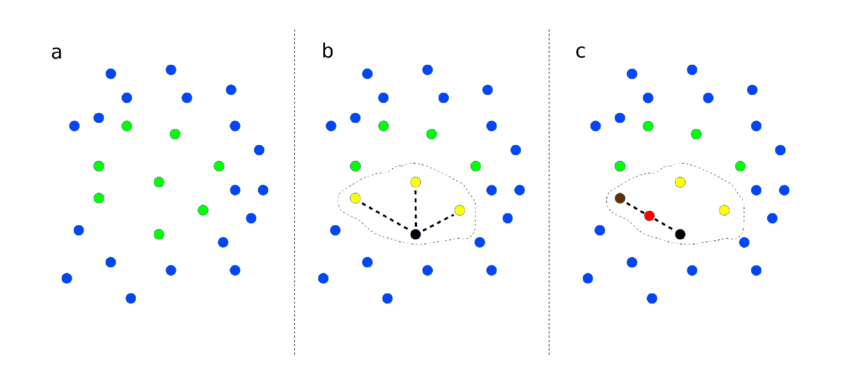
\includegraphics[width=0.7\textwidth]{figures/smote}
\caption{Graphical representation of the SMOT algorithm.}
\label{fig:smote}
\end{figure}

In \texttt{python} SMOT is implemented in \texttt{imblearn.over\_sampling} module.

\begin{ipython}
from imblearn.over_sampling import SMOTE
	
oversample = SMOTE()
X_sm, y_sm = oversample.fit_resample(X, y)
print (y_sm.value_counts())
\end{ipython}
\begin{ioutput}
1    6599
0    6599
Name: Bankrupt?, dtype: int64
\end{ioutput}

The last step to prepare the dataset for the analysis is its normalization which is necessary since each column ranges very differently.

\begin{ipython}
from sklearn.preprocessing import StandardScaler
from sklearn.model_selection import train_test_split
	
X_train, X_test, y_train, y_test = train_test_split(X_sm, y_sm,
                                                    test_size=0.2)
scaler = StandardScaler()
X_train = scaler.fit_transform(X_train)
X_test = scaler.transform(X_test)
\end{ipython}

%\begin{attention}
%Note that the \texttt{stratify} parameter creates batches of the dataset with the same proportion between the classes. While \texttt{random\_state} set the seeds for the random number generation for simpler debugging.
%\end{attention}

Now we can define the neural network architecture and go on with the training. An early stopping \emph{callback} has been implemented in order to stop the training in case no significant improvement is observed in the last 50 epochs in terms of loss reduction.

In computer programming, a callback is any executable code that is passed as an argument to other code; that other code is expected to execute at a given time.

\begin{ipython}
from tensorflow.keras.models import Sequential
from tensorflow.keras.layers import Dense, Dropout
from tensorflow.keras.callbacks import EarlyStopping
	
model = Sequential()
	
model.add(Dense(units=77, activation='relu'))
model.add(Dropout(0.3))
model.add(Dense(units=77, activation='relu'))
model.add(Dropout(0.3))
model.add(Dense(units=1, activation='sigmoid'))
	
model.compile(loss='binary_crossentropy', optimizer='adam')
	
early_stop = EarlyStopping(monitor='val_loss', 
                           mode='min', 
                           verbose=1, 
                           patience=50)
	
model.fit(x=X_train, y=y_train,
          epochs=600,
          validation_data=(X_test, y_test), 
          verbose=1, callbacks=[early_stop])
\end{ipython}
\begin{ioutput}
Epoch 1/600
330/330 [==============================] - 2s 4ms/step - loss: 0.3348 
- val_loss: 0.2354
Epoch 2/600
330/330 [==============================] - 1s 3ms/step - loss: 0.2318 
- val_loss: 0.2007
...
330/330 [==============================] - 2s 5ms/step - loss: 0.0148 
- val_loss: 0.0896
Epoch 00082: early stopping
\end{ioutput}

\begin{ipython}
loss = model.history.history['loss']
val_loss = model.history.history['val_loss']
\end{ipython}

Figure~\ref{fig:bankruptcy_loss} reports the loss function values, in training and testing samples, versus the epoch number. From the plot it is clear how there is no significant improvement after epoch 30 in the testing sample, that's why the training is stopped early.

\begin{figure}[htbp]
\centering
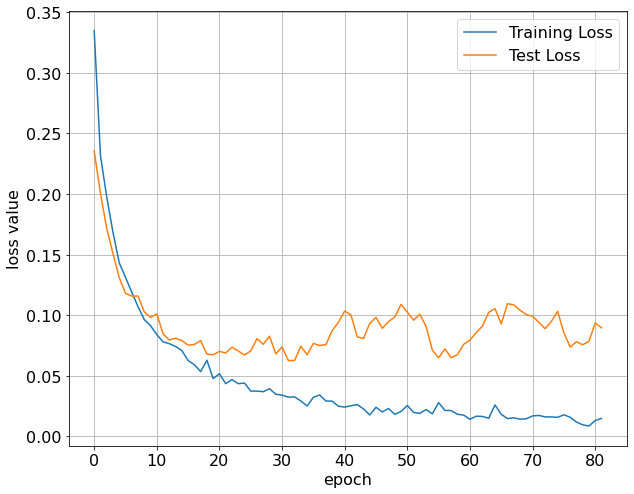
\includegraphics[width=0.7\linewidth]{figures/bankruptcy_loss}
\caption{Loss value as a function of the number of epochs in training and testing sample.}
\label{fig:bankruptcy_loss}
\end{figure}

Performance-wise the ANN can be evaluated using the so called \emph{confusion matrix} plot shown in Figure~\ref{fig:confusion_matrix}. This is a matrix that compares the number of actual and predicted events in each category, reporting true and false predictions. In case of two classes it becomes:

\begin{equation*}
	\begin{bmatrix}
		TP & FP \\
		FN & TN  
	\end{bmatrix}
\end{equation*}
\noindent
where $TP$ are the true "positive", $FN$ false "negative" and so on.

\begin{ipython}
from sklearn.metrics import confusion_matrix, ConfusionMatrixDisplay
	
ann_predictions = (model.predict(X_test) > 0.5).astype("int32")
	
cm = confusion_matrix(y_test, ann_predictions)
cmd_obj = ConfusionMatrixDisplay(cm, display_labels=['No Bankruptcy', 'Bankruptcy'])
cmd_obj.plot()
cmd_obj.ax_.set(title='', xlabel='Predicted', ylabel='Actual')
plt.show()
\end{ipython}
\noindent
From this matrix a number of information can be determined~\cite{bib:sensitivity}:

\makegapedcells\begin{table}[htbp]
\centering
\begin{tabular}{|l|c|c|}
\hline
Mis-classification (error rate) & $\cfrac{FP+FN}{n}$ & 0.8\% \\
\hline
Sensitivity (true positive) & $\cfrac{TP}{FN+TP}$ & 99.9 \% \\
\hline
False positive & $\cfrac{FP}{TN+FP}$ & 1.5\% \\
\hline
Specificity (true negative) & $\cfrac{TN}{TN+FP}$ &  98.5\% \\
\hline
False negative & $\cfrac{FN}{TP+FN}$ & 0.08\% \\
\hline
Precision & $\cfrac{TP}{FP+TP}$ & 98.4\% \\ 
\hline
Accuracy & $\cfrac{TN+TP}{n}$ & 99.2\% \\
\hline
\end{tabular}
\end{table}

\begin{figure}[htbp]
\centering
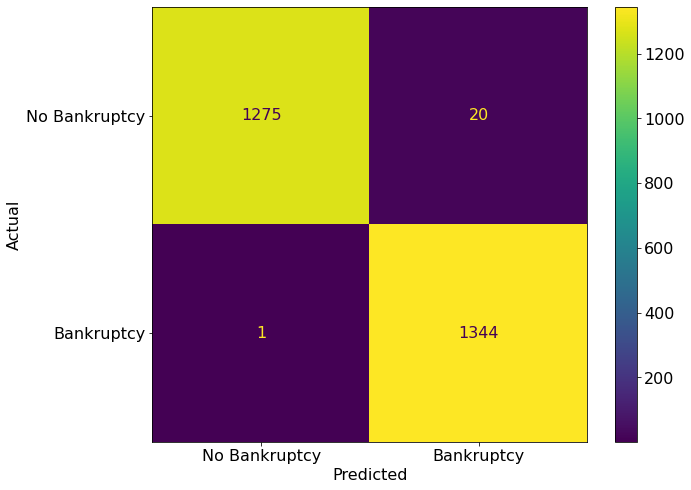
\includegraphics[width=0.7\linewidth]{figures/confusion_matrix}
\caption{Confusion matrix for the evaluation of the ANN to predict bankruptcy events.}
\label{fig:confusion_matrix}
\end{figure}

Since the goal was to train a neural network to predict company bankruptcy the most interesting parameters are the \emph{specificity} which is pretty high (98.5\%) and the \emph{false negative rate} which contrary is very small ($\lt 0.1\%$).

\section{Neural net to recognize handwritten digits}
\label{neural-net-to-recognize-handwritten-digits}

The difficulties of visual pattern recognition becomes immediately apparent if you attempt to write a computer program to recognize digits like those in Fig.~\ref{fig:mnist}.

\begin{figure}[b]
\centering
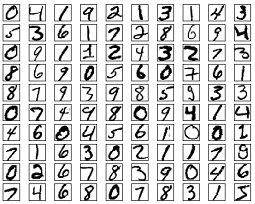
\includegraphics[width=0.5\textwidth]{figures/mnist_100_digits}
\caption{MNIST sample of handwritten digits.}
\label{fig:mnist}
\end{figure}

Simple intuition about how we discern shapes (e.g. a 9 has a loop at the top, and a vertical stroke in the bottom right) turns out to be not so simple to express algorithmically. When you try to make such rules precise, you quickly get lost in a morass of exceptions, caveats, and special cases so that it seems hopeless.

Neural networks approach the problem in a different way. They take a large number of handwritten digits and develop a system which can learn from those.

By increasing the number of training examples, the network can learn more and more about handwriting, and so improve its accuracy. So while it has been shown just 100 training digits in Fig.~\ref{fig:mnist}, a better handwriting recognizer could be certainly built by using thousands or millions training examples (\textbf{as we have seen above neural nets are not capable of extrapolating results, hence in general it won't recognize a digit written in some strange way not included in the training sample !!!}).

To explore the neural network capabilities the sample provided with the \texttt{mnist} module will be used. 
The algorithm is based on a different kind of neural network, specifically designed for image/pattern recognition, the Convolutional Neural Network (CNN). We won't go into the details of its implementation since it is outside the scope of these Chapter but it works by using different kind of layers (\emph{convolutional layers}) which apply various filters on top of the image, and each of them working as edge detectors. With them images are classified according to their features.

Stacking convolutional layers prove to be very effective, and allows to learn both low (e.g. lines) and high level features (e.g. lines, complex shapes or even specific objects), see Fig.~\ref{fig:conv_filters}.

\begin{figure}[htb]
\centering
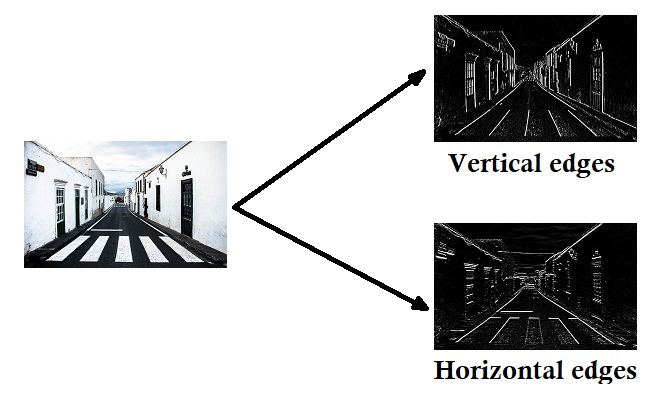
\includegraphics[width=1.\textwidth]{figures/edges.jpg}
\caption{Edge detected by different layers of a convolutional neural network.}
\label{fig:conv_filters}
\end{figure}

The CNN output won't be a single number but rather a list containing the probabilities that an image belongs to each class.

\begin{ipython}
import numpy as np, mnist
from finnn import FinNN

# the actual
train_images = mnist.train_images()
# the target
train_labels = mnist.train_labels() # (it is a 0, 1, 2...)

# no test_size option means not split the sample
# in training and testing sets
# (MNIST has already dont it for us)

trainer = FinNN("CNN2D")
trainer.setData(train_images, train_labels)
\end{ipython}
\noindent
Next we define the CNN architecture, see Fig.~\ref{fig:cnn2d}.

\begin{ipython}
# define our convolutional NN
# we decide to apply 8 filters to the images
# each with 3x3 pixels size
# the input images have 28x28 pixels size instead
trainer.addConv2DLayer(filters=8, filter_size=3, input_shape=(28, 28, 1))
trainer.addMaxPooling2D(2)
trainer.addFlatten()
trainer.addCNNOutputLayer(outputs=10)

trainer.compileModel(loss='categorical_crossentropy', opt='adam')
trainer.fit(epochs=5, verbose=1)
trainer.saveModel('digit_training')
\end{ipython}
\begin{ioutput}
Epoch 1/5
59999/59999 [==============================] - 13s 210us/step - loss: 2.1711
Epoch 2/5
59999/59999 [==============================] - 12s 201us/step - loss: 0.3964
Epoch 3/5
59999/59999 [==============================] - 12s 199us/step - loss: 0.2655
Epoch 4/5
59999/59999 [==============================] - 12s 198us/step - loss: 0.2244
Epoch 5/5
59999/59999 [==============================] - 12s 196us/step - loss: 0.1910
\end{ioutput}

\begin{figure}[htb]
\centering
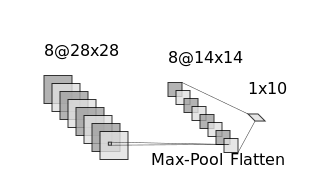
\includegraphics[width=0.9\textwidth]{figures/cnn_2d.png}
\caption{Graphical representation of the CNN developed to recognize handwritten digits.}
    \label{fig:cnn2d}
\end{figure}

\begin{attention}
\subsubsection{Pooling}

Looking closely to the convolutional neural network implementation we can notice new kind of layers never used before, in particular the \texttt{MaxPooling2} layer.

Convolutional layers in a CNN systematically apply filters to input images in order to create feature maps that summarize the main characteristics of the sample.

A limitation of such maps is that they record the precise position of features in the input. This means that small movements in its position will result in a different feature map. This can happen with cropping, rotation, shifting, and other minor changes to the input image.

Imagine a program that looks for car plates in pictures taken by a speed radar: cars won't be in the same position in the frame so there may be differences in the classification of similar (but not equal) pictures.

A common approach to address this problem is called \emph{down sampling}. 
This is where a lower resolution version of an input signal (e.g. the picture) is created that still contains the large or important structural elements, without the finer detail that may not be as useful to the task.

Down sampling can be achieved using a pooling layer.
It involves selecting kind of a filter to be applied to the feature maps. The pooling operation size is smaller than the feature map; specifically, it is almost always 2×2 pixels. This means that the pooling layer will always reduce the size of each feature map by a factor of 2, e.g. each dimension is halved. For example, a pooling layer applied to a feature map of 6×6 (36 pixels) will result in an output pooled feature map of 3×3 (9 pixels).

The most common pooling operation are:
\begin{itemize}
\tightlist
\item Average Pooling: calculate the average value for each patch on the feature map;
\item Maximum Pooling (or Max Pooling): calculate the maximum value for each patch of the feature map.
\end{itemize}
\end{attention}

Let's see how well our NN predicts \texttt{mnist} testing digits.

\begin{ipython}
trainer.loadModel('digit_training')
# testing with mnist test sample
test_images = mnist.test_images()
test_labels = mnist.test_labels()
trainer.setTestData(test_images, test_labels)
predictions = trainer.predict(trainer.x_test[:10])

print ("Tesing on MNIST digits...")
print("Predicted: ", np.argmax(predictions, axis=1))
print("Truth:", test_labels[:10])
print("highest prob.:", ["{:.3f}".format(p[np.argmax(p)]) for p in predictions])
\end{ipython}
\begin{ioutput}
Tesing on MNIST digits...
Predicted:  [7 2 1 0 4 1 4 4 5 9]
Truth: [7 2 1 0 4 1 4 9 5 9]
highest prob.: ['1.000', '1.000', '1.000', '1.000', '1.000', '0.999', 
'0.970', '0.900', '0.841', '0.999']
\end{ioutput}

Since the last but one digit has lower probability let's check the returned list to see which other number have non-zero probability.

\begin{ipython}
for i, p in enumerate(predictions[8])])
    print("9th digit:", ["dig {}: {:.3f}".format(i, p)
\end{ipython}
\begin{ioutput}
9th digit: ['dig 0: 0.000', 'dig 1: 0.000', 'dig 2: 0.000', 'dig 3: 0.000', 
'dig 4: 0.000', 'dig 5: 0.841', 'dig 6: 0.159', 'dig 7: 0.000', 
'dig 8: 0.000', 'dig 9: 0.000']
\end{ioutput}

So the second ranked digit is a 6 (which can be confused with a five if the lower loop is almost closed).

The NN performance can be checked using your own calligraphy. 

Open your favourite image editor (e.g. Paint, GIMP,\ldots) and create a black-white 200x200 pixels canvas. With the help of the mouse draw a digit and save it as a png file.
Before passing the image to the NN it has to be resized and this is done with an ad-hoc function, \texttt{transform\_image}, which can be imported from \href{https://raw.githubusercontent.com/matteosan1/finance_course/develop/libro/input_files/digit_converter.py}{\texttt{digit\_converter.py}}.

\begin{ipython}
from digit_converter import transform_image

filenames = ['four.png', 'five.png']
for f in filenames:
    test_images = np.array(transform_image(f))
test_images = np.expand_dims(test_images, axis=3)
predict = trainer.predict(test_images)

print ("Tesing on custom digits...")
print ("Predicted: ", np.argmax(predict, axis=1))
print("%:", ["{:.3f}".format(p[np.argmax(p)]) for p in predict])
print(["{:.2f}".format(p) for p in predict[0]])
\end{ipython}
\begin{ioutput}
Tesing on custom digits...
Predicted:  [4]
%: ['0.802']
['0.00', '0.00', '0.00', '0.00', '0.80', '0.00', '0.00', '0.20', '0.00', 
'0.00']

Testing on custom digits...
Predicted:  [5]
%: ['0.981']
['0.00', '0.00', '0.00', '0.01', '0.00', '0.98', '0.00', '0.01', '0.00', 
'0.00']
\end{ioutput}
The handwritten images used in this test are shown in Fig.~\ref{fig:test_images}.

\begin{figure}[htb]
\centering
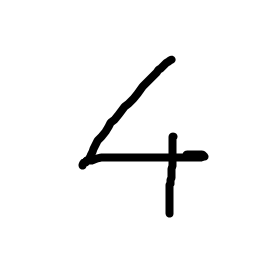
\includegraphics[width=0.2\textwidth]{figures/four.png}
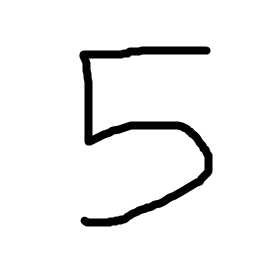
\includegraphics[width=0.2\textwidth]{figures/five.png}
\caption{Test handwritten digits used in the example.}
\label{fig:test_images}
\end{figure}

%\subsection{Model Calibration cont.}
%\label{model-calibration-cont.}
%
%When a model has just three known parameters a convolutional neural network can be used to calibrate it.
%
%Consider again the Black-Scholes formula and imagine you need to calibrate: rate $r$ and volatility $\sigma$ at the same time.
%
%A black-white image can be interpreted as a map where each pixel coordinates is a pair ($\mathrm{ttm}, M$) and the pixel color, an integer between 0 (black) and 255 (white), represents \(P_\textrm{call}\). Each picture will be classified by a pair of $r, \sigma$.
%
%The creation of the training sample is a little more complicated now. For convenience we will use also a new format to save data image, \texttt{numpy}. This will be done through the corresponding module simply using the functions \texttt{save} and \texttt{load} to store and retrieve data. The module \texttt{PIL} (\texttt{pillow}) is instead used to visualize the images.
%
%First make the targets.
%
%\begin{ipython}
%import numpy as np
%from finmarkets import call_m
%
%labels = []
%rates = np.arange(0.01, 0.11, 0.001)
%vols = np.arange(0.1, 0.6, 0.005)
%for i in range(len(vols)):
%    for j in range(len(rates)):
%        labels.append((vols[i], rates[j]))
%\end{ipython}
%\noindent
%Then we can create the images.
%
%\begin{ipython}
%k = np.arange(0.8, 1.2, (1.2-0.8)/20)
%ttm = np.arange(1, 5, 4/20)
%
%# for each r, sigma pair
%# generate a matrix of prices
%maximum = 0
%minimum = np.inf
%prices = []
%for v in vols:
%    for r in rates:
%        price = np.zeros(shape=(20, 20))
%        for ik, kv in enumerate(k):
%            for it, t in enumerate(ttm):
%                price[ik, it] = call_m(kv, r, v, t)
%                prices.append(price)
%                # max and min are saved to
%                # normalize our matrices
%                new_max = np.max(price)
%                new_min = np.min(price)
%                if new_max > maximum:
%                    maximum = new_max
%                if new_min < minimum:
%                    minimum = new_min
%for ip, p in enumerate(prices):
%    prices[ip] = np.interp(p, (minimum, maximum), (0, 1))
%np.save("2d", prices)
%\end{ipython}
%\noindent
%An example of the 20x20 images that have been created is shown in Fig.~\ref{fig:test_images_calib}.
%
%\begin{figure}[htb]
%\centering
%
\includegraphics[width=0.45\textwidth]{figures/2d_training_images}
%\caption{Example of images used to encode calibration information.}
%\label{fig:test_images_calib}
%\end{figure}
%\noindent
%Then the training is similar to what has been done for the handwritten digits.
%
%\begin{ipython}
%import numpy as np
%from finnn import FinNN
%
%labels = np.load("2d_labels.npy")
%images = np.load("2d.npy")
%
%trainer = FinNN("CNN2D")
%trainer.setData(images, labels, test_size=0.2)
%trainer.addConv2DLayer(filters=8, filter_size=10,
%                       input_shape=(20, 20, 1), activation='relu')
%trainer.addFlatten()
%trainer.addHiddenLayer(neurons=10, activation='relu')
%trainer.addOutputLayer(outputs=2, activation='relu')
%
%trainer.compileModel(loss='mse', opt='adam')
%trainer.fit(epochs=500, verbose=1)
%trainer.saveModel("2d")
%trainer.evaluate()
%\end{ipython}
%\begin{ioutput}
%Epoch 1/500
%8000/8000 [==============================] - 1s 156us/step - loss: 0.0018
%Epoch 2/500
%8000/8000 [==============================] - 1s 142us/step - loss: 6.2310e-04
%...
%Epoch 499/500
%8000/8000 [==============================] - 2s 194us/step - loss: 1.4921e-06
%Epoch 500/500
%8000/8000 [==============================] - 2s 193us/step - loss: 1.4413e-06
%
%8000/8000 [==============================] - 1s 65us/step
%Training: 1.1013161047230825e-05
%2000/2000 [==============================] - 0s 70us/step
%Test: 1.116331470257137e-05
%\end{ioutput}
%
%At this point the test of the trained CNN consists of presenting the prices of call referring to the same underlying in the pictorial form shown before and in response it will give the risk-free rate and the volatility.
%
%\begin{ipython}
%for i in range(5):
%    print (trainer.predict(trainer.x_test[i:i+1]))
%\end{ipython}
%\begin{ioutput}
%[[0.3825101  0.09229672]]
%[[0.4056808  0.02232919]]
%[[0.47402808 0.05630913]]
%[[0.2851617  0.05214534]]
%[[0.17245176 0.08815573]]
%\end{ioutput}

\section{Technical Analysis}
\label{technical-analysis}

In finance \emph{technical analysis} is a discipline for forecasting the direction of prices through the study of past market data, primarily price and volume. The analyst looks for particular patterns in the price time series that are \emph{believed} to develop in a predictable way. Fig.~\ref{fig:tech_ana} shows two of such patterns.

\begin{figure}[htb]
\centering
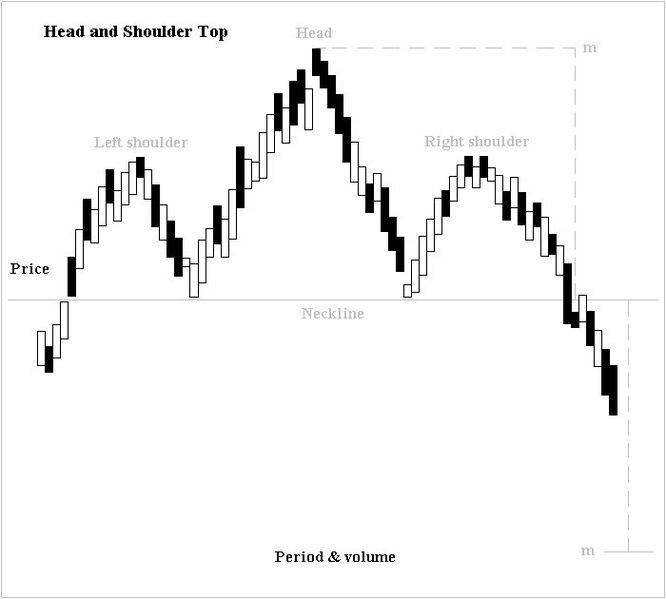
\includegraphics[width=0.4\linewidth]{figures/H_and_s_top_new.jpg}\qquad
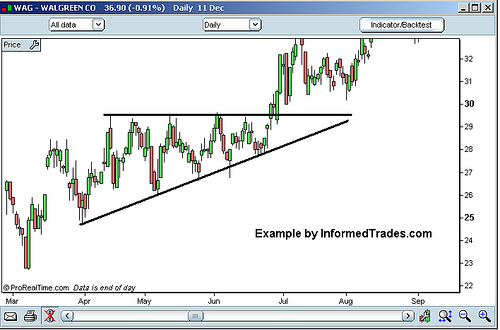
\includegraphics[width=0.4\linewidth]{figures/Triangle-ascending.jpg}
\caption{Examples of patterns in real time series, head and shoulder (left), triangle (right).}
\label{fig:tech_ana}
\end{figure}

We will develop a CNN capable of classifying features in time series to be used in technical analysis (which is much faster than having somebody looking at thousands of time series by eye).

The training sample is made of 21600 time series (1/3 with head and shoulder patter, 1/3 with triangle pattern and 1/3 with no pattern), see Fig~\ref{fig:patterns}. \textbf{To make the training easier the features are quite exaggerated.}

\begin{figure}[htbp]
\centering
\subfloat[No pattern.\label{}]{%
	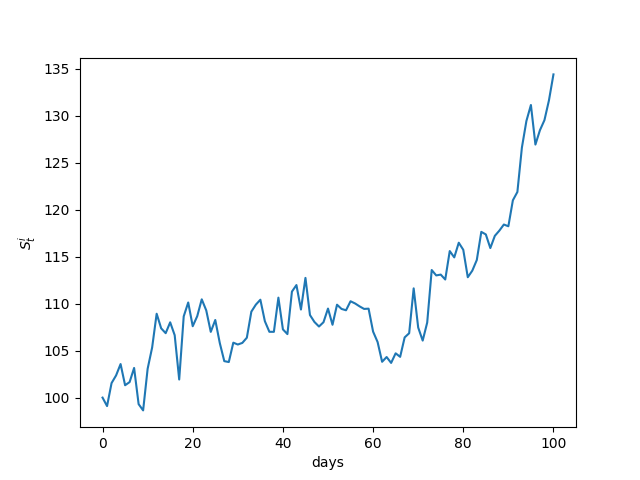
\includegraphics[width=0.5\textwidth]{figures/no_pattern}
}
\subfloat[Head and shoulder pattern.\label{}]{%
	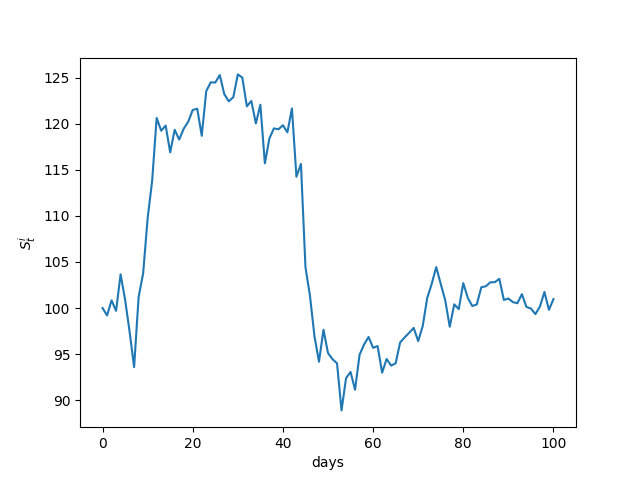
\includegraphics[width=0.5\textwidth]{figures/head_and_shoulder}
}\\
\subfloat[Triangle pattern.\label{}]{%
	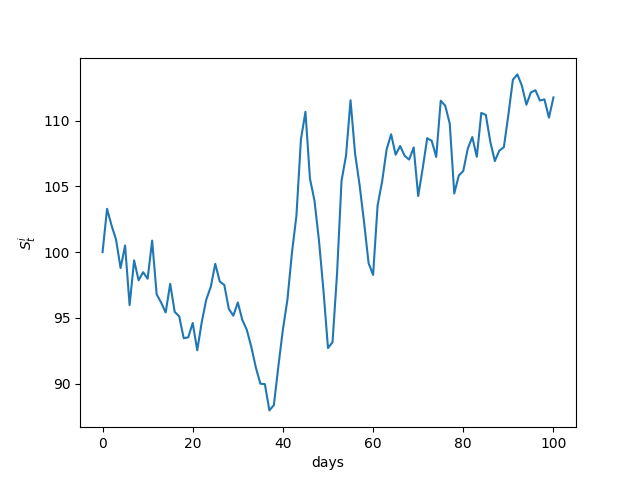
\includegraphics[width=0.5\textwidth]{figures/triangle}
}
\caption{Examples of time series used in the training of the CNN for technical analysis.}
\label{fig:patterns}
\end{figure}

\begin{ipython}
import numpy as np
from finnn import FinNN

train_labels = np.load("training_techana_labels.npy")
train_images = np.load("training_techana_images.npy")
trainer = FinNN("CNN1D")
trainer.setData(train_images, train_labels)

# define the CNN
trainer.addConv1DInputLayer(filters=80, filter_size=20,
                            input_size=(101, 1))
trainer.addConv1DLayer(filters=80, filter_size=15)
trainer.addMaxPooling1D(3)
trainer.addConv1DLayer(filters=100, filter_size=10)
trainer.addConv1DLayer(filters=100, filter_size=5)
trainer.addGlobalAveragePooling1D()
trainer.addDropout(0.5)
trainer.addCNNOutputLayer(outputs=3)

trainer.compileModel(loss='categorical_crossentropy', opt='adam')
trainer.fit(epochs=80)
trainer.saveModel('techana')
\end{ipython}
\begin{ioutput}
Epoch 1/80
- 23s 1ms/step - loss: 0.6773
Epoch 2/80
- 23s 1ms/step - loss: 0.5421
...
Epoch 79/80
- 23s - loss: 0.0737
Epoch 80/80
- 23s - loss: 0.0692
\end{ioutput}

\begin{attention}
\subsubsection{Dropout}

Large neural nets trained on relatively small datasets tend to overfit.

In this case the model is learning the statistical noise in the training data, so it results in poor performance when the model is evaluated on new data (e.g. the test dataset).

One approach to reduce overfitting is to fit all possible different neural networks on the same dataset and to average the predictions from each model. This is not feasible in practice, and can be approximated using a small collection of different models, called an ensemble. A problem even with the ensemble approximation is that it requires multiple models to be fit and stored, which can be a challenge if the models are large, requiring days or weeks to train and tune.

\emph{Dropout} is a regularization method that approximates training a large number of neural networks with different architectures in parallel.

During training, some number of layer outputs are randomly ignored or \emph{dropped out}. This has the effect of making the layer look like and treated like a layer with a different number of nodes and connectivity to the prior layer. In effect, each update to a layer during training is performed with a different "view" of the configured layer.

Even if it may seems counter intuitive (better training when switching off nodes) indeed dropout breaks up situations where network layers co-adapt to correct mistakes from prior layers, in turn making the model more robust.
\end{attention}

The NN performance are checked simulating a real case scenario where a time series is analyzed in "real-time" with the goal of recognizing any incoming pattern (the sooner, the better). 

The simulation is carried on presenting to the CNN sliding time windows
\begin{itemize}
	\item at $t_1$ the input is represented by the time series point between \([0, 80]\);
	\item at $t_2$ by the points between \([1, 81]\);
	\item at $t_3$ between \([2, 82]\) and so on.
\end{itemize}

Figure~\ref{fig:frame_simulation} shows the "temporal frames" that have been presented to the CNN.

\begin{figure}
\centering
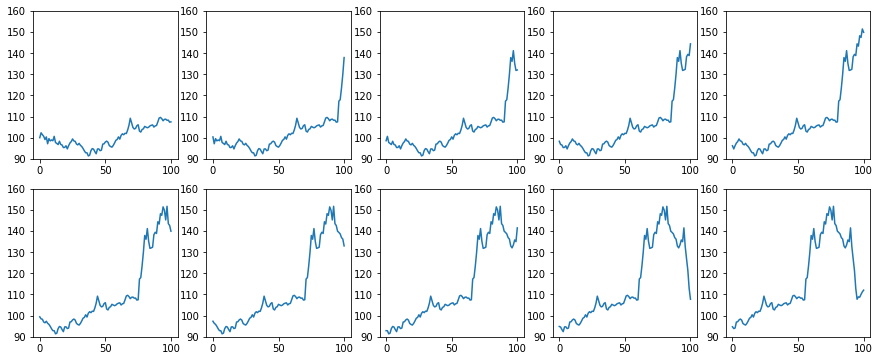
\includegraphics[width=\textwidth]{figures/tech_ana_frames}
\caption{Ten frames simulating closing price data incoming in real time. The CNN was tested to check if and when it would have been able to detect any pattern in data.}
\label{fig:frame_simulation}
\end{figure}

\begin{ipython}
test_images = np.load("testing_techana_frames.npy")
trainer.loadModel("techana")
predictions = trainer.predict(test_images)

for i in range(len(predictions)):
    print (np.argmax(predictions[i]), ["{:.3f}".format(p) for p in predictions[i]])
\end{ipython}
\begin{ioutput}
0 ['0.942', '0.000', '0.058']
0 ['0.970', '0.000', '0.030']
0 ['1.000', '0.000', '0.000']
0 ['0.999', '0.001', '0.000']
0 ['0.784', '0.216', '0.000']
1 ['0.000', '1.000', '0.000']
1 ['0.000', '1.000', '0.000']
1 ['0.000', '1.000', '0.000']
1 ['0.000', '1.000', '0.000']
1 ['0.000', '1.000', '0.000']
\end{ioutput}
\noindent
The output represents the likelihood that the time series  belong to any category at give times. Up to $t=4$ the CNN is more about 95\% sure there is no pattern (max probability at category 0). 
At $t=5$ the CNN starts to recognize a pattern assigning about 20\% probability to the "head and shoulders" class. For $t\geq 6$ the neural network recognizes the pattern with a probability close to 100\%.

\section{Unsupervised Learning}
    
Unsupervised learning is a type of machine learning in which the algorithm is not provided with any pre-assigned labels or scores for the training data.As a result, unsupervised learning algorithms must first self-discover any naturally occurring patterns in that training data set. 
    
Common examples include \emph{clustering}, where the algorithm automatically groups its training examples into categories with similar features, and principal component analysis~\ref{sec:pca}, where the algorithm finds ways to compress the training data set by identifying which features are most useful for discriminating between different training examples, and discarding the rest. 
    
\subsection{k-Means Algorithm}
    
k-means clustering is a method of vector quantization that aims to partition (split) $n$ observations into $k$ clusters in which each observation belongs to the cluster with the nearest mean (cluster centers or cluster centroid), serving as a prototype of the cluster. 
    
Given a set of observations $(x_1, x_2, \ldots, x_n)$, where each observation is a $d$-dimensional real vector, the algorithm divided the $n$ observations into $k$ $(\leq n)$ sets $S = \{S_1, S_2, \ldots, S_k\}$ so as to minimize the within-cluster sum of squares (WCSS) (i.e. variance). Formally, the objective is to find:
    
\begin{equation}
\underset {\mathbf {S}}{\operatorname {arg\,min} } \sum _{i=1}^{k}\sum _{\mathbf {x} \in S_{i}}\left\|\mathbf {x} -{\boldsymbol {\mu }}_{i}\right\|^{2}
\end{equation}
where $μ_i$ is the mean of points in $S_i$. 
    
\subsubsection{Example}
This example consists of clustering a dataset that contains information of all the stocks that compose the SP500 Index. 
    
The input dataset, fetched from Yahoo Finance and stored in \href{https://github.com/matteosan1/finance_course/raw/develop/libro/input_files/k\_mean.csv}{k\_mean.csv}, consists of the daily closing prices of each share within the interval 2018-09-20, 2021-09-20.
    
The goal of the project is to find similarities amongst companies in terms of return and volatility. To do this, the k-means clustering algorithm will produce labels that assign each company to different clusters.
 
The first step consists in loading the inputs and then produce a new \texttt{DataFrame} with annualized returns and volatilities for each stock. 
 
\begin{ipython}
import pandas as pd
 
df = pd.read_csv("k_mean.csv", index_col='Date')
 
returns = df.pct_change().mean() * 252
std = df.pct_change().std() * np.sqrt(252)
 
ret_var = pd.concat([returns, std], axis = 1).dropna()
ret_var.columns = ["Returns","Standard Deviation"]
print (ret_var.head())
\end{ipython}
\begin{ioutput}
       Returns  Standard Deviation
MMM  -0.188903            0.261649
ABT   0.235801            0.232519
ABBV -0.159596            0.304667
ABMD -0.543486            0.526830
ACN   0.152511            0.212579
\end{ioutput}

\subsection{Elbow Curve}
 
In order to determine the optimal number of clusters $k$ for our dataset, we will fit different models of the k-means algorithm while varying the $k$ parameter in the range 2 to 14. For each model we calculate the Sum Squared Error (SSE) by using the \texttt{.inertia\_\_} method of the fitted model (inertia tells how far away the points within a cluster are. The smaller the inertia value the better).
 
Each pair of values ($k$, SSE) will help to construct the \emph{Elbow Curve} which can be used to determine the optimal value for $k$. 
 
Using the "elbow" or "knee" of a curve as a cutoff point is a common heuristic in mathematical optimization to choose a point where diminishing returns are no longer worth the additional cost. In clustering, this means one should choose a number of clusters so that adding another cluster doesn't give much better modeling of the data.
 
The intuition is that increasing the number of clusters will naturally improve the fit (explain more of the variation) since there are more parameters (more clusters) to use, but at some point this becomes over-fitting, and the elbow reflects this. 
 
In practice there may not be a sharp elbow, and as a heuristic method, such an "elbow" cannot always be unambiguously identified.

The k-means method is implemented in the \texttt{sklearn.cluster.KMeans} class.

\begin{ipython} 
from sklearn.cluster import KMeans
 
X =  ret_var.values 
sse = []
for k in range(2, 15):
    kmeans = KMeans(n_clusters = k)
    kmeans.fit(X)
   
    sse.append(kmeans.inertia_) 
\end{ipython}

\begin{figure}
\centering
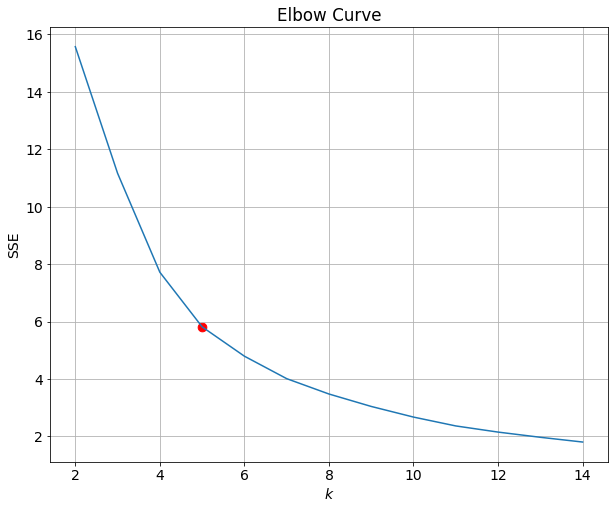
\includegraphics[width=0.7\textwidth]{figures/elbow_curve}
\caption{The eblow curve for the studied example.}
\label{fig:elbow_curve}
\end{figure}
 
The resulting graph of Fig.~\ref{fig:elbow_curve} shows that the optimal value of $k$ is 5.

\begin{ipython} 
kmeans = KMeans(n_clusters = 5).fit(X)
centroids = kmeans.cluster_centers_
\end{ipython}

\begin{figure}
\centering
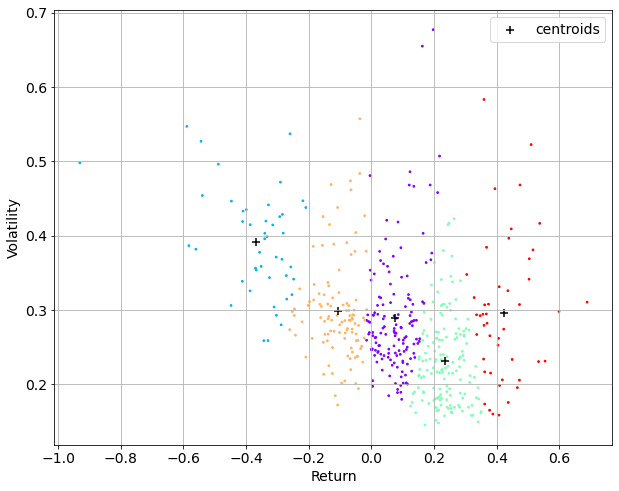
\includegraphics[width=0.7\textwidth]{figures/k_means_5}
\caption{The clustering results with the parameter $k$ equal to 5.}
\label{fig:K_means_5}
\end{figure}
 
Fig.~\ref{fig:elbow_curve} shows also the presence of outliers as only one point is on the upper right side of the graph. This outlier form its own cluster. In order to have a better categorization of the stocks within the SP500 index, we would remove those stocks and fit the model another time.
This is done by finding the stock with the highest standard deviation value and dropping the corresponding columnn.
 
\begin{ipython}
stdOrder = ret_var.sort_values('Standard Deviation', ascending=False)
first_symbol = stdOrder.index[0]
ret_var.drop(first_symbol, inplace=True)
\end{ipython}
Then we can fit the dataset again, Fig.~\ref{fig:k_means_noout} reports the result.

\begin{ipython}
X = ret_var.values
kmeans = KMeans(n_clusters = 5).fit(X)
centroids = kmeans.cluster_centers_
\end{ipython}
 
\begin{figure}
\centering
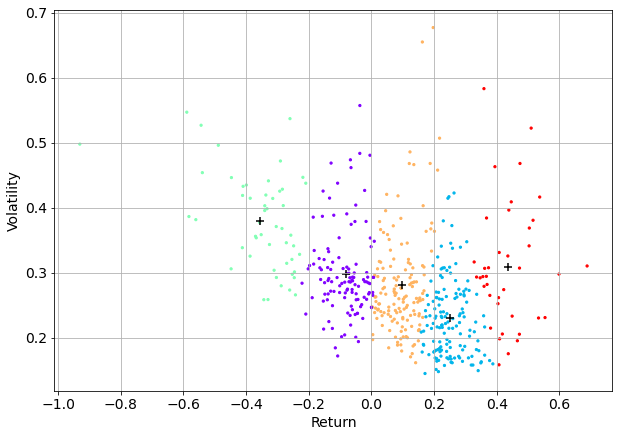
\includegraphics[width=0.7\textwidth]{figures/k_means_noout}
\caption{The clustering results after the outliers removal.}
\label{fig:K_means_noout}
\end{figure}
  
Finally we will assign to each stock it correspondent number of cluster(1,2,3,4,and 5) and make a \texttt{DataFrame} with this information. Having the information of cluster number for each stock, we can create a diversified portfolio in the long term, between stocks from different clusters.

\begin{ipython} 
stocks = pd.DataFrame(ret_var.index) # the dataframe structure allow concatenation
cluster_labels = pd.DataFrame(kmeans.labels_)
stockClusters = pd.concat([stocks, cluster_labels],axis = 1)
stockClusters.columns = ['Symbol','Cluster']
\end{ipython}
 
As an example the following are the stocks belonging to cluster number 0.

\begin{ipython} 
print (stockClusters.loc[stockClusters['Cluster'] == 0, 'Symbol'])
\end{ipython}
\begin{ioutput}
6      ADBE
7       AMD
11        A
14      ALK
20      ALL
       ... 
465    VRTX
466     VFC
483     WDC
493     XYL
496     ZBH
Name: Symbol, Length: 145, dtype: object
\end{ioutput}
 
\begin{thebibliography}{9}
\bibitem{bib:deep_learning} I. Goodfellow, Y. Bengio and A. Courville, \href{http://www.deeplearningbook.org}{\emph{Deep Learning}}, MIT Press, 2016
\bibitem{bib:nn_over_human}K. Grace, J. Salvatier, A. Dafoe, B. Zhang and O. Evans, \emph{When Will AI Exceed Human Performance? Evidence from AI Experts}, arXiv:1705.08807, 2005
\bibitem{bib:activation_function} J. Lederer, \emph{Activation Functions in Artificial Neural Networks: A Systematic Overview}, arxiv: 2101.09957, 2001
\bibitem{bib:backpropagation}\href{https://towardsdatascience.com/understanding-backpropagation-algorithm-7bb3aa2f95fd}{\emph{Understanding back-propagation algorithm}}, Towards Data Science [Online]
\bibitem{bib:loss_function}\href{https://medium.com/human-in-a-machine-world/mae-and-rmse-which-metric-is-better-e60ac3bde13d}{\emph{Mae and rmse which metric is better ?}}, Medium [Online]
\bibitem{bib:keras}\href{https://keras.io/}{\emph{Keras Documentation}}, [Online]  
\bibitem{bib:tensorflow}\href{https://www.tensorflow.org/}{\emph{Tensorflow Documentation}}, [Online] 
\bibitem{bib:scikit}\href{https://scikit-learn.org/stable/}{\emph{scikit-learn Documentation}}, [Online]
\bibitem{bib:smot}Nitesh Chawla, et al., \emph{SMOTE: Synthetic Minority Over-sampling Technique.}, 2012
\bibitem{bib:sensitivity}\href{https://en.wikipedia.org/wiki/Sensitivity_and_specificity}{\emph{Sensitivity and specificity}}, [Online]
\end{thebibliography}